\chapter{Primer on UAVs}
\label{ch:uav-primer}

This chapter presents background information on unmanned aerial vehicles
(UAVs), or drones. Drones have had a long history of evolution, starting as
huge gunnery targets in the 1910s to today's small consumer photography drones
which are readily available in stores. Beginning with the history of their
evolution in \cref{sec:drone-history}, we move on to describe the capabilities
found in present-day drones in \cref{sec:drone-capabilities}. We end in
\cref{sec:autonomy-levels} with a description of a framework for characterizing
autonomous capabilities in drones.

\section{History of Drones}
\label{sec:drone-history}

\begin{figure}[htbp]
\centerline{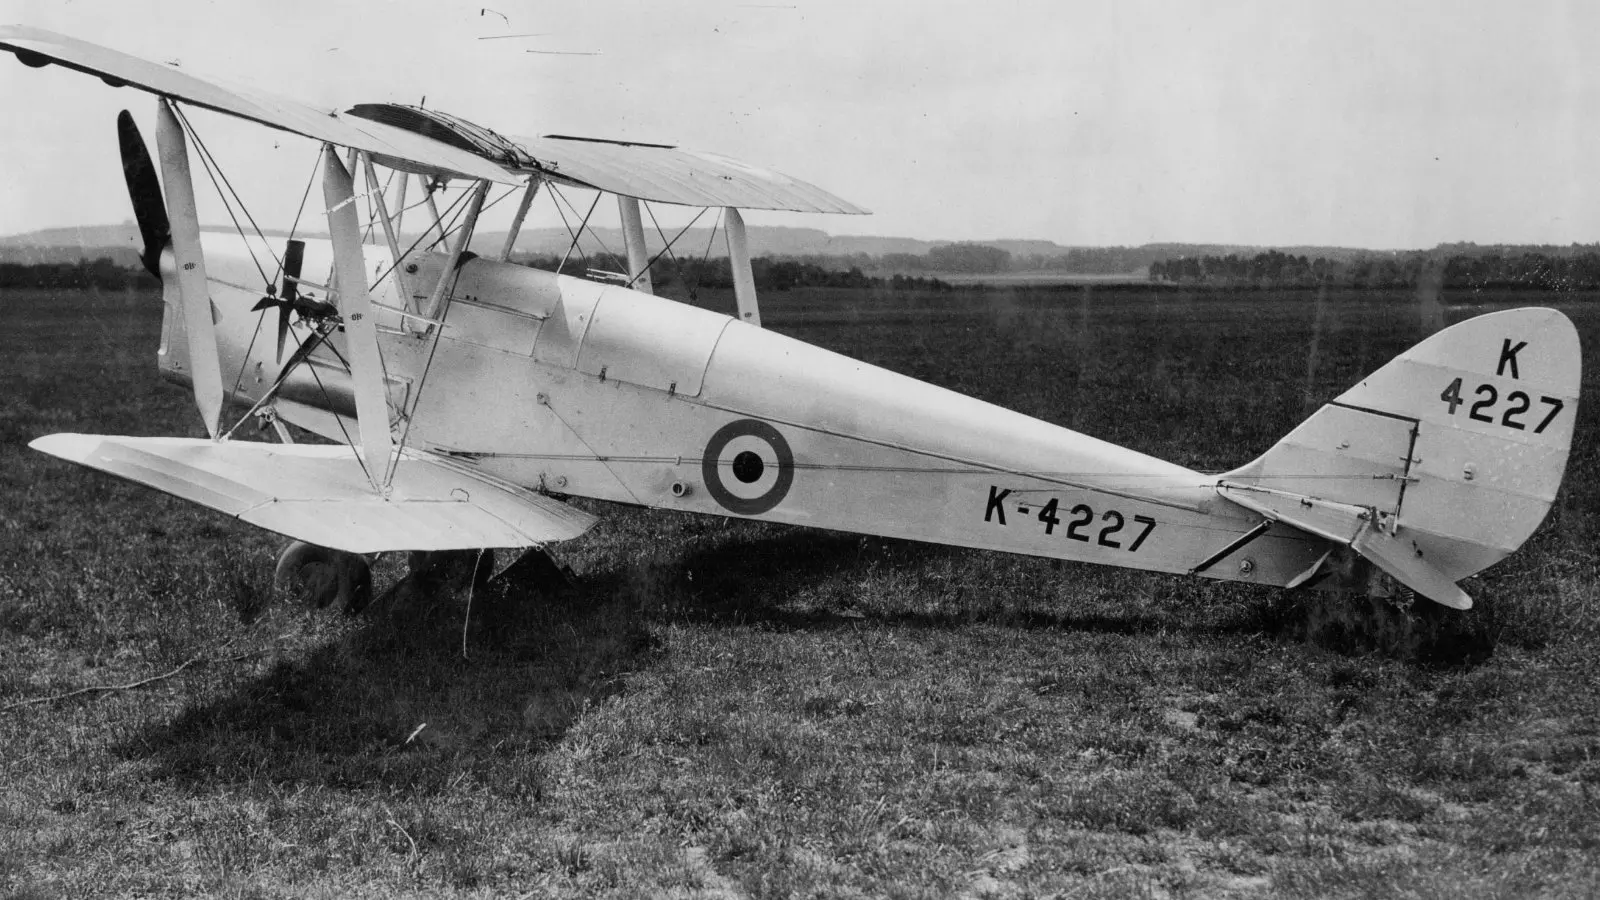
\includegraphics[width = .6\textwidth]{figs/queenbee.png}}
\caption{de Havilland DH82B Queen Bee \cite{baesystems}, the first radio-controlled drone}
\label{fig:queen-bee}
\end{figure}

Drones, are aircraft that can be operated remotely without the need for a human
pilot on board. While there were many early pilotless aircraft, the first
remote controlled aircraft appeared during the First World War, developed by
Britain and the US in 1917 \cite{dronehistory}. Many of these early drones were
used as anti-aircraft gunnery training targets. In the 1930s, the term "drone"
arose inspired by the de Havilland DH82B Queen Bee (\cref{fig:queen-bee}),
designed as a low-cost radio-controlled target aircraft, which saw over four
hundred units built by 1943. The Queen Bee was the first drone designed with
the ability to return to ground safely and be reused \cite{queenbee, pbs05}.

These early drones were fixed-wing aircraft that were used primarily for combat
or training. From the 1970s, drones such as the Ryan Model 147 Lightning
Bugdrones were developed for use in surveillance missions. These drones carried
a camera and could fly for hours at high altitude \cite{pbs12}. The Pioneer
UAV, introduced in 1986, saw extensive use in the Gulf War. Today, the General
Atomics MQ-1 Predator can fly for over 14 hours performing surveillance
missions using an array of sensors, including infrared cameras.

\begin{figure}[htbp]
\centerline{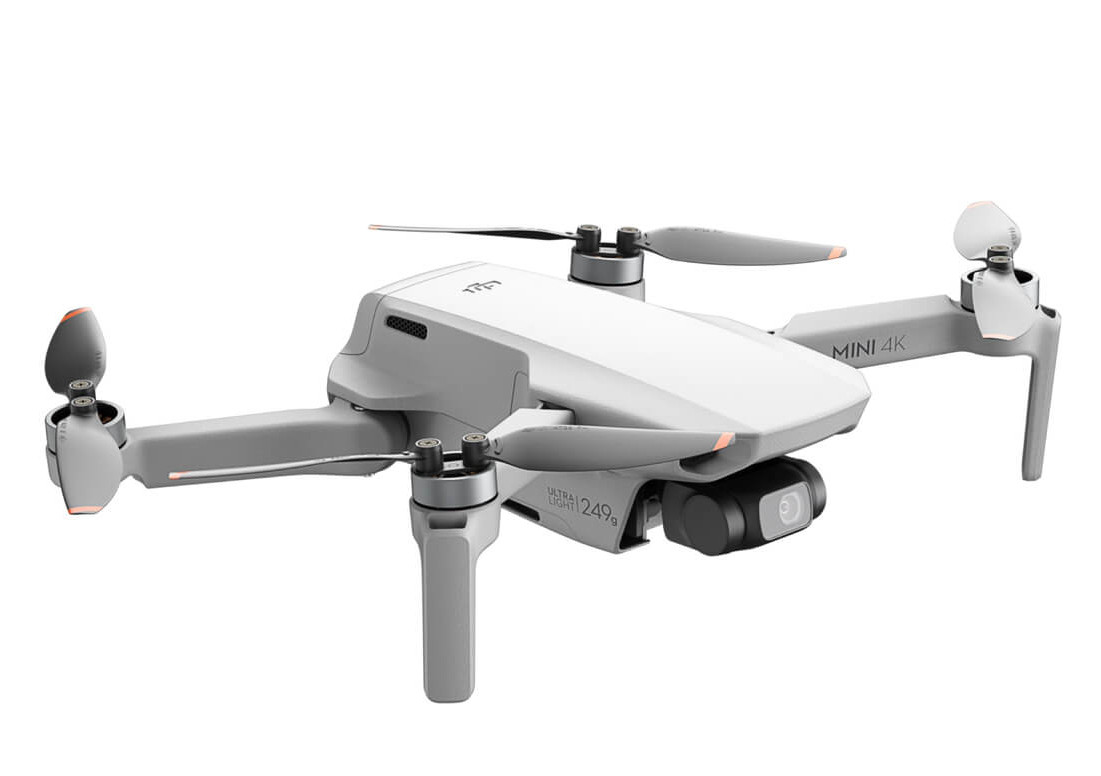
\includegraphics[width = .3\textwidth]{figs/dji-mini-4k.jpg}}
\caption{DJI Mini 4K}
\label{fig:dji-mini-4k}
\end{figure}

The turn of the century saw the use of small drones in civillian settings, with
technology advances making them cheaper to produce. Drones, particularly
quadcopters (\cref{fig:dji-mini-4k}), started being used for mapping, aerial
photography, industrial inspections and security, and precision agriculture
\cite{giones2017}. Compared to previous fixed-wing military drones, quadcopters
offer superior maneuverability and the ability to hover. They utilize four
motor-rotors, with two spinning clockwise and the other two counterclockwise.
Variations in motor speed allow for precise hovering and maneuverability. This
makes quadcopter drones well-suited for both indoor and outdoor use.  Since the
2010s, drones have evolved significantly, with a range of consumer photography
and racing drones easily available to consumers, at a wide range of price
points. Drones are commonly used for filming and recreation, and have also seen
use in logistics, to deliver packages. They have also been put to use in search and rescue
\cite{scherer2015}\cite{tomic2012}\cite{mcrae2019} and wildlife conservation \cite{gemert2015}\cite{gonzalez2016}.

The scale of their adoption is
immense---The Federal Aviation Administration (FAA) has received registrations
for almost 800,000 drones \cite{faa_drones_2024}.  This figure excludes
thousands of hobbyist drones weighing under 250 g that do not require FAA
registration.

\section{Capabilities of Present-day Drones}
\label{sec:drone-capabilities}

Today, the set of features available in consumer-grade drones is impressive.
The DJI Mini 4K (\cref{fig:dji-mini-4k}) is priced at \$299, weighs under 250g,
records video at 4K 30 FPS, and has a maximum flight time of about 30 minutes
\cite{dji_mini_4k}. Most drone's today have the ability to fly
semi-autonomously in addition to the ability to be controlled remotely by a
human. As shown in \cref{fig:drone-components}, drones have advanced
microprocessors that abstract away the lower-level mechanics of quadcopter
drone flight. Components such as the Electronic Speed Controller (ESC) enable
precise control of the drone's brushless electric motors. On-board positioning
systems such as Global Navigation Satellite System (GNSS) receivers give the
drone the ability to navigate between waypoints.  Using inputs from on-board
intertial measurement unit (IMU) sensors such as gyroscopes, accelerometers,
and magnetometers, drones can determine their orientation, acceleration, and
rotation, allowing them to adjust their motors in real-time to counter wind and
hover in a fixed position. They can also typically takeoff and land
autonomously. On-board flight control software such as PX4 or ArduPilot, also
known as an "autopilot," makes these higher-level functions possible, taking
inputs from the IMU and GNSS sensors and outputting control commands to the
ESC.

\begin{figure}[htbp]
\centerline{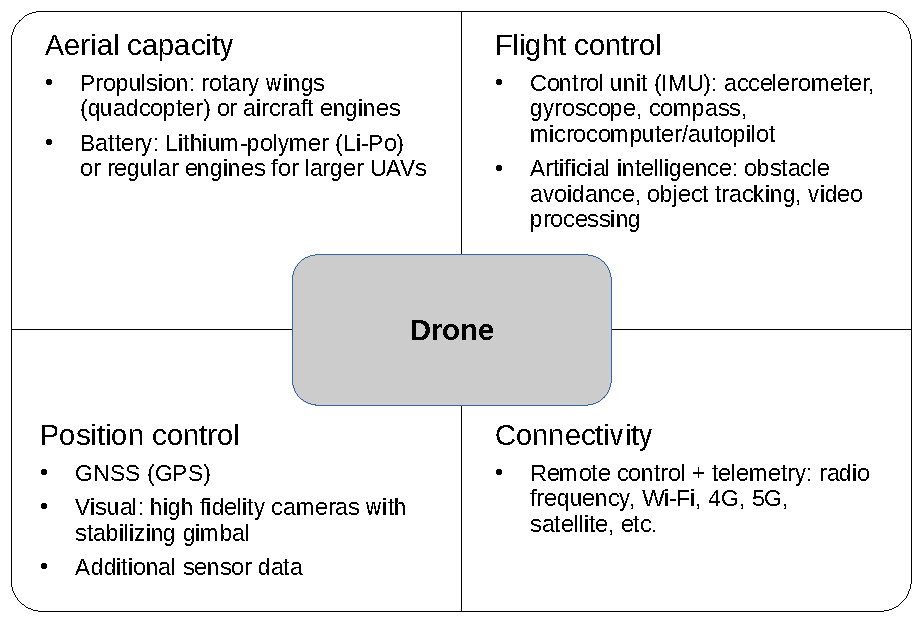
\includegraphics[width = .6\textwidth]{figs/drone-components-crop.pdf}}
\caption{Components of a drone \cite{giones2017}}
\label{fig:drone-components}
\end{figure}

Drones are equipped with a variety of cameras, such as monocular and stereo.
Monocular cameras capture images and videos from a single point of view, and
are common in consumer aerial photography drones. Monocular cameras are often
mounted on a gimbal, which stabilizes the drone's camera during motion and also
allows the ability to capture different viewing angles through gimbal motion.
Stereoscopic cameras, on the other hand, offer multiple point of views. Having
more than one camera allows the use of epipolar geometry and triangulation to
determine distance from objects efficiently, and perform obstacle avoidance.
The DJI Mini 4 Pro, for instance, has multiple binocular cameras, facing
forward, backward, sideways, upwards, and downwards. This allows the Mini 4 Pro
to perform omnidirectional obstacle sensing. During manual pilot flight, the
drone offers pilot assistance features that stop the drone if it is headed for
an imminent collision, and also provide the option to circumvent obstacles
automatically altogether. Drones equipped with monocular cameras typically lack
these advanced obstacle avoidance systems, but are cheaper and more common.

While consumer-grade drones offer many semi-autonomous features, complex
fully-autonomous features are limited to more expensive commerical drones.  For
example, a consumer drone could be instructed to navigate to a given GPS
coordinate or, in some advanced drones, even track an on-ground target. But
complex missions, such as patrolling a set of waypoints while searching for an
on-ground target, and transitioning to track the target once it is detected,
remain out of the reach of consumer drones.

Consumer drones are typically controlled over Wi-Fi using a controller or a
smartphone app, and typically lack cellular connectivity, limiting their
flying range.

\section{Levels of Drone Autonomy}
\label{sec:autonomy-levels}

\begin{figure}[htbp]
\centerline{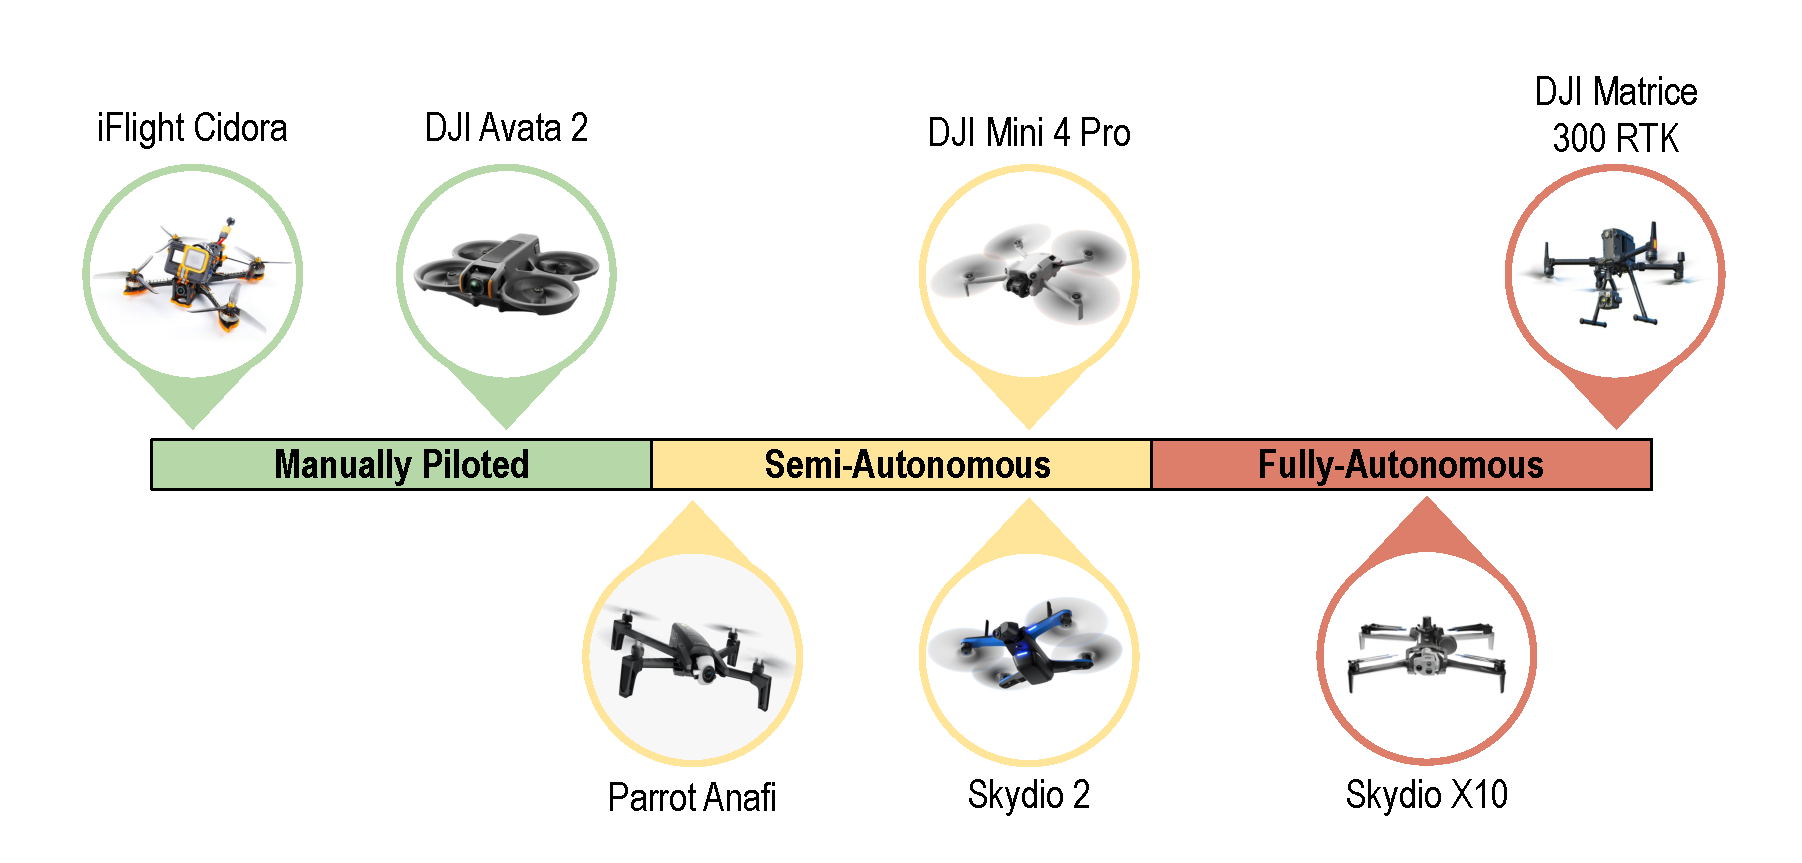
\includegraphics[width = .8\textwidth]{figs/autonomy-spectrum.pdf}}
\caption{Drone Autonomy Levels}
\label{fig:drone-autonomy-spectrum}
\end{figure}

Drones exhibit varying levels of autonomy, as shown in
\cref{fig:drone-autonomy-spectrum}. As we move to the right, the reliance on
human drone operators reduces, as the drones feature more autonomous abilities.
On the manual end of the spectrum are drones such as the DJI Avata 2, a
first-person view (FPV) drone. FPV drone pilots receive a real-time video
stream from the drone's onboard camera and manually control the drone. These
drones are optimized for high-speed flight and maneuverability, giving them the
ability to navigate through tight obstacles at speed. Manually piloting a drone
requires skill and constant human pilot input, which reduces the usefulness of
these drones.

Drones such as the Parrot Anafi include semi-autonomous features such as the
ability to hover and navigate between waypoints. These drones often include a
return-to-home (RTH) function which automatically returns the drone to its
takeoff location if the battery is low, or if the drone loses its connection to
the pilot's controller. Advanced semi-autonomous drones such as the DJI Mini 4
Pro can also follow a human or vehicle target. These semi-autonomous features
reduce the level of skill required for piloting and the reliance on the human
pilot, but still require the pilot to specify the next course of action to
fulfill higher-level mission objectives.

\begin{figure}[htbp]
    \centerline{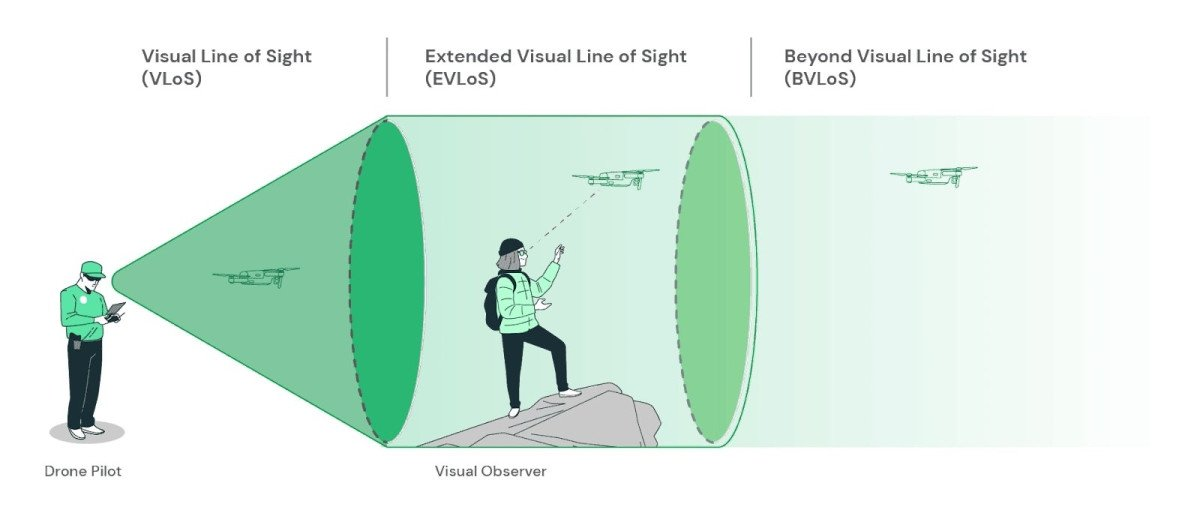
\includegraphics[width = .9\textwidth]{figs/BVLOS.jpeg}}
    \caption{Drone Operation Line-of-Sight Requirements \cite{flyeye_bvlos}}
\label{fig:drone-line-of-sight}
\end{figure}

On the right end of the spectrum are fully-autonomous drones, which execute a
pre-programmed mission without a human pilot while adapting to operational and
environmental conditions during flight. The DJI Matrice 300 RTK, for instance,
can inspect pre-specified objects of interest, such as power transmission
towers, without any human input.

Regulatory hurdles, however, impact the versatility of fully-autonomous drones.
FAA regulations require that drone operators keep drones within sight during
flight \cite{faa_part107}. For FPV drones, it is sufficient to have a visual
observer that always has the drone in sight.  These two modes of operation
correspond to ``Visual Line of Sight'' (VLoS) and ``Extended Visual Line of
Sight'' (EVLoS) in \cref{fig:drone-line-of-sight}. While a number of use cases
can be covered under these modes of operation, the holy grail for drones lies
in ``Beyond Visual Line of Sight'' (BVLoS) operation. BVLoS operation allows
drones to fly a much wider range of missions. Missions involve package delivery
requires drones to fly to a far-off destination, improving speed and reducing
the logistical cost compared to human delivery via road. Requiring a human
observer to maintain sight of the drone at all times defeats the purpose of
this application.
